\begin{center}
	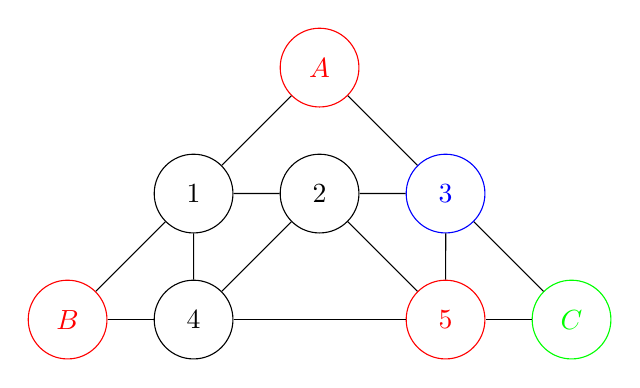
\begin{tikzpicture}[scale=1.6]
		\tikzset{nd/.style={circle, draw=black, minimum width=1cm}};

		\node[nd, red] (a) at (2, 2) {$A$};
		\node[nd] (1) at (1, 1) {$1$};
		\node[nd] (2) at (2, 1) {$2$};
		\node[nd, blue] (3) at (3, 1) {$3$};
		\node[nd, red] (b) at (0, 0) {$B$};
		\node[nd] (4) at (1, 0) {$4$};
		\node[nd, red] (5) at (3, 0) {$5$};
		\node[nd, green] (c) at (4, 0) {$C$};

		\draw (a) to (1);
		\draw (a) to (3);

		\draw (1) to (2);
		\draw (1) to (b);
		\draw (1) to (4);

		\draw (2) to (3);
		\draw (2) to (4);
		\draw (2) to (5);

		\draw (3) to (5);
		\draw (3) to (c);

		\draw (b) to (4);

		\draw (4) to (5);

		\draw (5) to (c);


	\end{tikzpicture}
\end{center}
